\documentclass[1p]{elsarticle_modified}
%\bibliographystyle{elsarticle-num}

%\usepackage[colorlinks]{hyperref}
%\usepackage{abbrmath_seonhwa} %\Abb, \Ascr, \Acal ,\Abf, \Afrak
\usepackage{amsfonts}
\usepackage{amssymb}
\usepackage{amsmath}
\usepackage{amsthm}
\usepackage{scalefnt}
\usepackage{amsbsy}
\usepackage{kotex}
\usepackage{caption}
\usepackage{subfig}
\usepackage{color}
\usepackage{graphicx}
\usepackage{xcolor} %% white, black, red, green, blue, cyan, magenta, yellow
\usepackage{float}
\usepackage{setspace}
\usepackage{hyperref}

\usepackage{tikz}
\usetikzlibrary{arrows}

\usepackage{multirow}
\usepackage{array} % fixed length table
\usepackage{hhline}

%%%%%%%%%%%%%%%%%%%%%
\makeatletter
\renewcommand*\env@matrix[1][\arraystretch]{%
	\edef\arraystretch{#1}%
	\hskip -\arraycolsep
	\let\@ifnextchar\new@ifnextchar
	\array{*\c@MaxMatrixCols c}}
\makeatother %https://tex.stackexchange.com/questions/14071/how-can-i-increase-the-line-spacing-in-a-matrix
%%%%%%%%%%%%%%%

\usepackage[normalem]{ulem}

\newcommand{\msout}[1]{\ifmmode\text{\sout{\ensuremath{#1}}}\else\sout{#1}\fi}
%SOURCE: \msout is \stkout macro in https://tex.stackexchange.com/questions/20609/strikeout-in-math-mode

\newcommand{\cancel}[1]{
	\ifmmode
	{\color{red}\msout{#1}}
	\else
	{\color{red}\sout{#1}}
	\fi
}

\newcommand{\add}[1]{
	{\color{blue}\uwave{#1}}
}

\newcommand{\replace}[2]{
	\ifmmode
	{\color{red}\msout{#1}}{\color{blue}\uwave{#2}}
	\else
	{\color{red}\sout{#1}}{\color{blue}\uwave{#2}}
	\fi
}

\newcommand{\Sol}{\mathcal{S}} %segment
\newcommand{\D}{D} %diagram
\newcommand{\A}{\mathcal{A}} %arc


%%%%%%%%%%%%%%%%%%%%%%%%%%%%%5 test

\def\sl{\operatorname{\textup{SL}}(2,\Cbb)}
\def\psl{\operatorname{\textup{PSL}}(2,\Cbb)}
\def\quan{\mkern 1mu \triangleright \mkern 1mu}

\theoremstyle{definition}
\newtheorem{thm}{Theorem}[section]
\newtheorem{prop}[thm]{Proposition}
\newtheorem{lem}[thm]{Lemma}
\newtheorem{ques}[thm]{Question}
\newtheorem{cor}[thm]{Corollary}
\newtheorem{defn}[thm]{Definition}
\newtheorem{exam}[thm]{Example}
\newtheorem{rmk}[thm]{Remark}
\newtheorem{alg}[thm]{Algorithm}

\newcommand{\I}{\sqrt{-1}}
\begin{document}

%\begin{frontmatter}
%
%\title{Boundary parabolic representations of knots up to 8 crossings}
%
%%% Group authors per affiliation:
%\author{Yunhi Cho} 
%\address{Department of Mathematics, University of Seoul, Seoul, Korea}
%\ead{yhcho@uos.ac.kr}
%
%
%\author{Seonhwa Kim} %\fnref{s_kim}}
%\address{Center for Geometry and Physics, Institute for Basic Science, Pohang, 37673, Korea}
%\ead{ryeona17@ibs.re.kr}
%
%\author{Hyuk Kim}
%\address{Department of Mathematical Sciences, Seoul National University, Seoul 08826, Korea}
%\ead{hyukkim@snu.ac.kr}
%
%\author{Seokbeom Yoon}
%\address{Department of Mathematical Sciences, Seoul National University, Seoul, 08826,  Korea}
%\ead{sbyoon15@snu.ac.kr}
%
%\begin{abstract}
%We find all boundary parabolic representation of knots up to 8 crossings.
%
%\end{abstract}
%\begin{keyword}
%    \MSC[2010] 57M25 
%\end{keyword}
%
%\end{frontmatter}

%\linenumbers
%\tableofcontents
%
\newcommand\colored[1]{\textcolor{white}{\rule[-0.35ex]{0.8em}{1.4ex}}\kern-0.8em\color{red} #1}%
%\newcommand\colored[1]{\textcolor{white}{ #1}\kern-2.17ex	\textcolor{white}{ #1}\kern-1.81ex	\textcolor{white}{ #1}\kern-2.15ex\color{red}#1	}

{\Large $\underline{12n_{0595}~(K12n_{0595})}$}

\setlength{\tabcolsep}{10pt}
\renewcommand{\arraystretch}{1.6}
\vspace{1cm}\begin{tabular}{m{100pt}>{\centering\arraybackslash}m{274pt}}
\multirow{5}{120pt}{
	\centering
	\includegraphics[width=112pt]{../../../GIT/diagram.site/Diagrams/png/2684_12n_0595.png}\\
\ \ \ A knot diagram\footnotemark}&
\allowdisplaybreaks
\textbf{Linearized knot diagam} \\
\cline{2-2}
 &
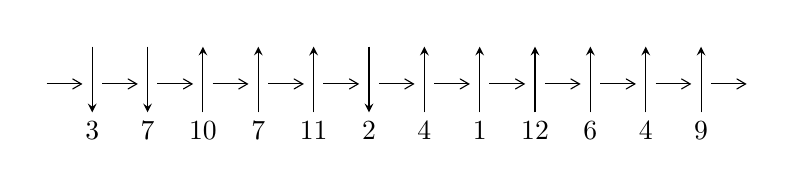
\begin{tikzpicture}[x=20pt, y=17pt]
	% nodes
	\node (C0) at (0, 0) {};
	\node (C1) at (1, 0) {};
	\node (C1U) at (1, +1) {};
	\node (C1D) at (1, -1) {3};

	\node (C2) at (2, 0) {};
	\node (C2U) at (2, +1) {};
	\node (C2D) at (2, -1) {7};

	\node (C3) at (3, 0) {};
	\node (C3U) at (3, +1) {};
	\node (C3D) at (3, -1) {10};

	\node (C4) at (4, 0) {};
	\node (C4U) at (4, +1) {};
	\node (C4D) at (4, -1) {7};

	\node (C5) at (5, 0) {};
	\node (C5U) at (5, +1) {};
	\node (C5D) at (5, -1) {11};

	\node (C6) at (6, 0) {};
	\node (C6U) at (6, +1) {};
	\node (C6D) at (6, -1) {2};

	\node (C7) at (7, 0) {};
	\node (C7U) at (7, +1) {};
	\node (C7D) at (7, -1) {4};

	\node (C8) at (8, 0) {};
	\node (C8U) at (8, +1) {};
	\node (C8D) at (8, -1) {1};

	\node (C9) at (9, 0) {};
	\node (C9U) at (9, +1) {};
	\node (C9D) at (9, -1) {12};

	\node (C10) at (10, 0) {};
	\node (C10U) at (10, +1) {};
	\node (C10D) at (10, -1) {6};

	\node (C11) at (11, 0) {};
	\node (C11U) at (11, +1) {};
	\node (C11D) at (11, -1) {4};

	\node (C12) at (12, 0) {};
	\node (C12U) at (12, +1) {};
	\node (C12D) at (12, -1) {9};
	\node (C13) at (13, 0) {};

	% arrows
	\draw[->,>={angle 60}]
	(C0) edge (C1) (C1) edge (C2) (C2) edge (C3) (C3) edge (C4) (C4) edge (C5) (C5) edge (C6) (C6) edge (C7) (C7) edge (C8) (C8) edge (C9) (C9) edge (C10) (C10) edge (C11) (C11) edge (C12) (C12) edge (C13) ;	\draw[->,>=stealth]
	(C1U) edge (C1D) (C2U) edge (C2D) (C3D) edge (C3U) (C4D) edge (C4U) (C5D) edge (C5U) (C6U) edge (C6D) (C7D) edge (C7U) (C8D) edge (C8U) (C9D) edge (C9U) (C10D) edge (C10U) (C11D) edge (C11U) (C12D) edge (C12U) ;
	\end{tikzpicture} \\
\hhline{~~} \\& 
\textbf{Solving Sequence} \\ \cline{2-2} 
 &
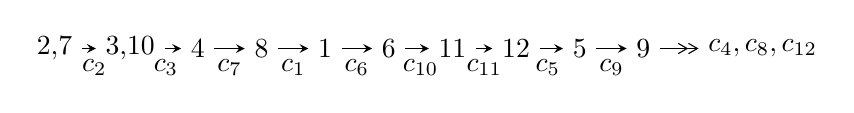
\begin{tikzpicture}[x=23pt, y=7pt]
	% node
	\node (A0) at (-1/8, 0) {2,7};
	\node (A1) at (17/16, 0) {3,10};
	\node (A2) at (17/8, 0) {4};
	\node (A3) at (25/8, 0) {8};
	\node (A4) at (33/8, 0) {1};
	\node (A5) at (41/8, 0) {6};
	\node (A6) at (49/8, 0) {11};
	\node (A7) at (57/8, 0) {12};
	\node (A8) at (65/8, 0) {5};
	\node (A9) at (73/8, 0) {9};
	\node (C1) at (1/2, -1) {$c_{2}$};
	\node (C2) at (13/8, -1) {$c_{3}$};
	\node (C3) at (21/8, -1) {$c_{7}$};
	\node (C4) at (29/8, -1) {$c_{1}$};
	\node (C5) at (37/8, -1) {$c_{6}$};
	\node (C6) at (45/8, -1) {$c_{10}$};
	\node (C7) at (53/8, -1) {$c_{11}$};
	\node (C8) at (61/8, -1) {$c_{5}$};
	\node (C9) at (69/8, -1) {$c_{9}$};
	\node (A10) at (11, 0) {$c_{4},c_{8},c_{12}$};

	% edge
	\draw[->,>=stealth]	
	(A0) edge (A1) (A1) edge (A2) (A2) edge (A3) (A3) edge (A4) (A4) edge (A5) (A5) edge (A6) (A6) edge (A7) (A7) edge (A8) (A8) edge (A9) ;
	\draw[->>,>={angle 60}]	
	(A9) edge (A10);
\end{tikzpicture} \\ 

\end{tabular} \\

\footnotetext{
The image of knot diagram is generated by the software ``\textbf{Draw programme}" developed by Andrew Bartholomew(\url{http://www.layer8.co.uk/maths/draw/index.htm\#Running-draw}), where we modified some parts for our purpose(\url{https://github.com/CATsTAILs/LinksPainter}).
}\phantom \\ \newline 
\centering \textbf{Ideals for irreducible components\footnotemark of $X_{\text{par}}$} 
 
\begin{align*}
I^u_{1}&=\langle 
187 u^{23}+2090 u^{22}+\cdots+32 b+20128,\;629 u^{23}+5916 u^{22}+\cdots+64 a+31616,\\
\phantom{I^u_{1}}&\phantom{= \langle  }u^{24}+10 u^{23}+\cdots+544 u+64\rangle \\
I^u_{2}&=\langle 
-5.02864\times10^{17} a^{11} u^{2}-2.22146\times10^{17} a^{10} u^{2}+\cdots-9.76070\times10^{17} a-5.75653\times10^{16},\\
\phantom{I^u_{2}}&\phantom{= \langle  }- a^{11} u^2-3 a^{10} u^2+\cdots+342 a+270,\;u^3- u^2+1\rangle \\
I^u_{3}&=\langle 
-7 u^{14}+17 u^{13}+\cdots+b-7,\;-7 u^{14}+14 u^{13}+\cdots+a-12,\\
\phantom{I^u_{3}}&\phantom{= \langle  }u^{15}-3 u^{14}+11 u^{12}-11 u^{11}-14 u^{10}+30 u^9+u^8-35 u^7+15 u^6+22 u^5-15 u^4-7 u^3+6 u^2+u-1\rangle \\
\\
\end{align*}
\raggedright * 3 irreducible components of $\dim_{\mathbb{C}}=0$, with total 75 representations.\\
\footnotetext{All coefficients of polynomials are rational numbers. But the coefficients are sometimes approximated in decimal forms when there is not enough margin.}
\newpage
\renewcommand{\arraystretch}{1}
\centering \section*{I. $I^u_{1}= \langle 187 u^{23}+2090 u^{22}+\cdots+32 b+20128,\;629 u^{23}+5916 u^{22}+\cdots+64 a+31616,\;u^{24}+10 u^{23}+\cdots+544 u+64 \rangle$}
\flushleft \textbf{(i) Arc colorings}\\
\begin{tabular}{m{7pt} m{180pt} m{7pt} m{180pt} }
\flushright $a_{2}=$&$\begin{pmatrix}1\\0\end{pmatrix}$ \\
\flushright $a_{7}=$&$\begin{pmatrix}0\\u\end{pmatrix}$ \\
\flushright $a_{3}=$&$\begin{pmatrix}1\\u^2\end{pmatrix}$ \\
\flushright $a_{10}=$&$\begin{pmatrix}-\frac{629}{64} u^{23}-\frac{1479}{16} u^{22}+\cdots-\frac{15951}{4} u-494\\-\frac{187}{32} u^{23}-\frac{1045}{16} u^{22}+\cdots-\frac{9705}{2} u-629\end{pmatrix}$ \\
\flushright $a_{4}=$&$\begin{pmatrix}\frac{1}{8} u^{23}+\frac{9}{8} u^{22}+\cdots+\frac{69}{2} u+\frac{9}{2}\\\frac{1}{8} u^{23}+\frac{5}{4} u^{22}+\cdots+\frac{129}{2} u+8\end{pmatrix}$ \\
\flushright $a_{8}=$&$\begin{pmatrix}\frac{11}{16} u^{23}+\frac{29}{4} u^{22}+\cdots+\frac{1881}{4} u+60\\-\frac{1}{8} u^{23}+\frac{1}{2} u^{22}+\cdots+383 u+52\end{pmatrix}$ \\
\flushright $a_{1}=$&$\begin{pmatrix}- u^2+1\\- u^4\end{pmatrix}$ \\
\flushright $a_{6}=$&$\begin{pmatrix}u\\u\end{pmatrix}$ \\
\flushright $a_{11}=$&$\begin{pmatrix}\frac{683}{64} u^{23}+\frac{1455}{16} u^{22}+\cdots+\frac{10705}{4} u+320\\\frac{469}{32} u^{23}+\frac{1889}{16} u^{22}+\cdots+\frac{3623}{2} u+185\end{pmatrix}$ \\
\flushright $a_{12}=$&$\begin{pmatrix}\frac{23}{16} u^{23}+\frac{83}{4} u^{22}+\cdots+2552 u+347\\-\frac{191}{16} u^{23}-\frac{1531}{16} u^{22}+\cdots-1486 u-148\end{pmatrix}$ \\
\flushright $a_{5}=$&$\begin{pmatrix}\frac{1}{8} u^{23}+\frac{9}{8} u^{22}+\cdots+\frac{69}{2} u+\frac{9}{2}\\\frac{1}{8} u^{23}+u^{22}+\cdots+30 u^2+\frac{9}{2} u\end{pmatrix}$ \\
\flushright $a_{9}=$&$\begin{pmatrix}-\frac{35}{16} u^{23}-\frac{83}{4} u^{22}+\cdots-\frac{3627}{4} u-112\\\frac{3}{8} u^{23}-\frac{1}{2} u^{22}+\cdots-905 u-124\end{pmatrix}$\\&\end{tabular}
\flushleft \textbf{(ii) Obstruction class $= -1$}\\~\\
\flushleft \textbf{(iii) Cusp Shapes $= 9 u^{23}+\frac{361}{4} u^{22}+\cdots+5492 u+734$}\\~\\
\newpage\renewcommand{\arraystretch}{1}
\flushleft \textbf{(iv) u-Polynomials at the component}\newline \\
\begin{tabular}{m{50pt}|m{274pt}}
Crossings & \hspace{64pt}u-Polynomials at each crossing \\
\hline $$\begin{aligned}c_{1}\end{aligned}$$&$\begin{aligned}
&u^{24}+10 u^{23}+\cdots+5120 u+4096
\end{aligned}$\\
\hline $$\begin{aligned}c_{2},c_{6}\end{aligned}$$&$\begin{aligned}
&u^{24}-10 u^{23}+\cdots-544 u+64
\end{aligned}$\\
\hline $$\begin{aligned}c_{3},c_{5},c_{10}\end{aligned}$$&$\begin{aligned}
&u^{24}+u^{22}+\cdots- u+1
\end{aligned}$\\
\hline $$\begin{aligned}c_{4},c_{7}\end{aligned}$$&$\begin{aligned}
&u^{24}+4 u^{23}+\cdots+3 u+1
\end{aligned}$\\
\hline $$\begin{aligned}c_{8},c_{9},c_{12}\end{aligned}$$&$\begin{aligned}
&u^{24}+6 u^{23}+\cdots+36 u+8
\end{aligned}$\\
\hline $$\begin{aligned}c_{11}\end{aligned}$$&$\begin{aligned}
&u^{24}-2 u^{23}+\cdots-253 u^2+16
\end{aligned}$\\
\hline
\end{tabular}\\~\\
\newpage\renewcommand{\arraystretch}{1}
\flushleft \textbf{(v) Riley Polynomials at the component}\newline \\
\begin{tabular}{m{50pt}|m{274pt}}
Crossings & \hspace{64pt}Riley Polynomials at each crossing \\
\hline $$\begin{aligned}c_{1}\end{aligned}$$&$\begin{aligned}
&y^{24}+10 y^{23}+\cdots+246415360 y+16777216
\end{aligned}$\\
\hline $$\begin{aligned}c_{2},c_{6}\end{aligned}$$&$\begin{aligned}
&y^{24}-10 y^{23}+\cdots-5120 y+4096
\end{aligned}$\\
\hline $$\begin{aligned}c_{3},c_{5},c_{10}\end{aligned}$$&$\begin{aligned}
&y^{24}+2 y^{23}+\cdots+3 y+1
\end{aligned}$\\
\hline $$\begin{aligned}c_{4},c_{7}\end{aligned}$$&$\begin{aligned}
&y^{24}-36 y^{23}+\cdots-43 y+1
\end{aligned}$\\
\hline $$\begin{aligned}c_{8},c_{9},c_{12}\end{aligned}$$&$\begin{aligned}
&y^{24}+20 y^{23}+\cdots-208 y+64
\end{aligned}$\\
\hline $$\begin{aligned}c_{11}\end{aligned}$$&$\begin{aligned}
&y^{24}-28 y^{23}+\cdots-8096 y+256
\end{aligned}$\\
\hline
\end{tabular}\\~\\
\newpage\flushleft \textbf{(vi) Complex Volumes and Cusp Shapes}
$$\begin{array}{c|c|c}  
\text{Solutions to }I^u_{1}& \I (\text{vol} + \sqrt{-1}CS) & \text{Cusp shape}\\
 \hline 
\begin{aligned}
u &= -0.960426 + 0.434752 I \\
a &= \phantom{-}1.39464 - 0.85244 I \\
b &= \phantom{-}0.96884 - 1.42503 I\end{aligned}
 & -0.39618 + 3.94424 I & \phantom{-}9.54953 - 8.49759 I \\ \hline\begin{aligned}
u &= -0.960426 - 0.434752 I \\
a &= \phantom{-}1.39464 + 0.85244 I \\
b &= \phantom{-}0.96884 + 1.42503 I\end{aligned}
 & -0.39618 - 3.94424 I & \phantom{-}9.54953 + 8.49759 I \\ \hline\begin{aligned}
u &= \phantom{-}0.148613 + 0.911725 I \\
a &= \phantom{-}0.535233 + 0.029034 I \\
b &= -0.053071 - 0.492300 I\end{aligned}
 & -3.90744 - 1.61982 I & \phantom{-}3.51812 + 4.40153 I \\ \hline\begin{aligned}
u &= \phantom{-}0.148613 - 0.911725 I \\
a &= \phantom{-}0.535233 - 0.029034 I \\
b &= -0.053071 + 0.492300 I\end{aligned}
 & -3.90744 + 1.61982 I & \phantom{-}3.51812 - 4.40153 I \\ \hline\begin{aligned}
u &= -0.610326 + 0.971717 I \\
a &= -0.759390 + 0.695247 I \\
b &= \phantom{-}0.212108 + 1.162240 I\end{aligned}
 & \phantom{-}3.60557 + 0.61915 I & \phantom{-}6.47955 - 0.75287 I \\ \hline\begin{aligned}
u &= -0.610326 - 0.971717 I \\
a &= -0.759390 - 0.695247 I \\
b &= \phantom{-}0.212108 - 1.162240 I\end{aligned}
 & \phantom{-}3.60557 - 0.61915 I & \phantom{-}6.47955 + 0.75287 I \\ \hline\begin{aligned}
u &= -0.603350 + 1.069910 I \\
a &= \phantom{-}0.600113 - 0.693104 I \\
b &= -0.379478 - 1.060250 I\end{aligned}
 & \phantom{-}6.67312 - 4.02157 I & \phantom{-}8.76645 + 3.55064 I \\ \hline\begin{aligned}
u &= -0.603350 - 1.069910 I \\
a &= \phantom{-}0.600113 + 0.693104 I \\
b &= -0.379478 + 1.060250 I\end{aligned}
 & \phantom{-}6.67312 + 4.02157 I & \phantom{-}8.76645 - 3.55064 I \\ \hline\begin{aligned}
u &= \phantom{-}1.242100 + 0.248561 I \\
a &= -0.058554 - 0.232893 I \\
b &= \phantom{-}0.014842 + 0.303830 I\end{aligned}
 & -2.22462 - 1.76771 I & -0.33207 + 2.72222 I \\ \hline\begin{aligned}
u &= \phantom{-}1.242100 - 0.248561 I \\
a &= -0.058554 + 0.232893 I \\
b &= \phantom{-}0.014842 - 0.303830 I\end{aligned}
 & -2.22462 + 1.76771 I & -0.33207 - 2.72222 I\\
 \hline 
 \end{array}$$\newpage$$\begin{array}{c|c|c}  
\text{Solutions to }I^u_{1}& \I (\text{vol} + \sqrt{-1}CS) & \text{Cusp shape}\\
 \hline 
\begin{aligned}
u &= -0.598153 + 1.149870 I \\
a &= -0.482510 + 0.665162 I \\
b &= \phantom{-}0.476234 + 0.952691 I\end{aligned}
 & \phantom{-}1.93569 - 8.47324 I & \phantom{-}4.22747 + 6.00356 I \\ \hline\begin{aligned}
u &= -0.598153 - 1.149870 I \\
a &= -0.482510 - 0.665162 I \\
b &= \phantom{-}0.476234 - 0.952691 I\end{aligned}
 & \phantom{-}1.93569 + 8.47324 I & \phantom{-}4.22747 - 6.00356 I \\ \hline\begin{aligned}
u &= -1.125790 + 0.732879 I \\
a &= \phantom{-}1.287760 - 0.541469 I \\
b &= \phantom{-}1.05292 - 1.55335 I\end{aligned}
 & \phantom{-}1.96046 + 5.63124 I & \phantom{-}4.21368 - 3.68677 I \\ \hline\begin{aligned}
u &= -1.125790 - 0.732879 I \\
a &= \phantom{-}1.287760 + 0.541469 I \\
b &= \phantom{-}1.05292 + 1.55335 I\end{aligned}
 & \phantom{-}1.96046 - 5.63124 I & \phantom{-}4.21368 + 3.68677 I \\ \hline\begin{aligned}
u &= -1.274940 + 0.470739 I \\
a &= -0.919966 + 0.816206 I \\
b &= -0.78868 + 1.47368 I\end{aligned}
 & -8.06206 + 6.43186 I & -0.98186 - 9.91203 I \\ \hline\begin{aligned}
u &= -1.274940 - 0.470739 I \\
a &= -0.919966 - 0.816206 I \\
b &= -0.78868 - 1.47368 I\end{aligned}
 & -8.06206 - 6.43186 I & -0.98186 + 9.91203 I \\ \hline\begin{aligned}
u &= -1.155680 + 0.779068 I \\
a &= -1.296620 + 0.435684 I \\
b &= -1.15905 + 1.51367 I\end{aligned}
 & \phantom{-}4.90945 + 10.68360 I & \phantom{-}6.29274 - 6.83109 I \\ \hline\begin{aligned}
u &= -1.155680 - 0.779068 I \\
a &= -1.296620 - 0.435684 I \\
b &= -1.15905 - 1.51367 I\end{aligned}
 & \phantom{-}4.90945 - 10.68360 I & \phantom{-}6.29274 + 6.83109 I \\ \hline\begin{aligned}
u &= -0.444487 + 0.406708 I \\
a &= -1.387950 + 0.186641 I \\
b &= -0.541015 + 0.647447 I\end{aligned}
 & \phantom{-}1.007530 - 0.240613 I & \phantom{-}10.53326 + 2.62206 I \\ \hline\begin{aligned}
u &= -0.444487 - 0.406708 I \\
a &= -1.387950 - 0.186641 I \\
b &= -0.541015 - 0.647447 I\end{aligned}
 & \phantom{-}1.007530 + 0.240613 I & \phantom{-}10.53326 - 2.62206 I\\
 \hline 
 \end{array}$$\newpage$$\begin{array}{c|c|c}  
\text{Solutions to }I^u_{1}& \I (\text{vol} + \sqrt{-1}CS) & \text{Cusp shape}\\
 \hline 
\begin{aligned}
u &= -1.18147 + 0.80593 I \\
a &= \phantom{-}1.276470 - 0.354607 I \\
b &= \phantom{-}1.22233 - 1.44770 I\end{aligned}
 & \phantom{-}0.0595 + 15.4273 I & \phantom{-}2.28436 - 8.54538 I \\ \hline\begin{aligned}
u &= -1.18147 - 0.80593 I \\
a &= \phantom{-}1.276470 + 0.354607 I \\
b &= \phantom{-}1.22233 + 1.44770 I\end{aligned}
 & \phantom{-}0.0595 - 15.4273 I & \phantom{-}2.28436 + 8.54538 I \\ \hline\begin{aligned}
u &= \phantom{-}1.56391 + 0.41904 I \\
a &= \phantom{-}0.060771 + 0.164825 I \\
b &= -0.025972 - 0.283237 I\end{aligned}
 & -8.02840 - 4.65058 I & -5.55122 + 0. I\phantom{ +0.000000I} \\ \hline\begin{aligned}
u &= \phantom{-}1.56391 - 0.41904 I \\
a &= \phantom{-}0.060771 - 0.164825 I \\
b &= -0.025972 + 0.283237 I\end{aligned}
 & -8.02840 + 4.65058 I & -5.55122 + 0. I\phantom{ +0.000000I}\\
 \hline 
 \end{array}$$\newpage\newpage\renewcommand{\arraystretch}{1}
\centering \section*{II. $I^u_{2}= \langle -5.03\times10^{17} a^{11} u^{2}-2.22\times10^{17} a^{10} u^{2}+\cdots-9.76\times10^{17} a-5.76\times10^{16},\;- a^{11} u^2-3 a^{10} u^2+\cdots+342 a+270,\;u^3- u^2+1 \rangle$}
\flushleft \textbf{(i) Arc colorings}\\
\begin{tabular}{m{7pt} m{180pt} m{7pt} m{180pt} }
\flushright $a_{2}=$&$\begin{pmatrix}1\\0\end{pmatrix}$ \\
\flushright $a_{7}=$&$\begin{pmatrix}0\\u\end{pmatrix}$ \\
\flushright $a_{3}=$&$\begin{pmatrix}1\\u^2\end{pmatrix}$ \\
\flushright $a_{10}=$&$\begin{pmatrix}a\\0.760828 a^{11} u^{2}+0.336105 a^{10} u^{2}+\cdots+1.47678 a+0.0870957\end{pmatrix}$ \\
\flushright $a_{4}=$&$\begin{pmatrix}0.161224 a^{11} u^{2}-0.231777 a^{10} u^{2}+\cdots-0.574135 a-1.02670\\0.322449 a^{11} u^{2}-0.463555 a^{10} u^{2}+\cdots-1.14827 a-2.05340\end{pmatrix}$ \\
\flushright $a_{8}=$&$\begin{pmatrix}-1.11863 a^{11} u^{2}-2.00948 a^{10} u^{2}+\cdots-0.0799198 a+0.987036\\-2.18025 a^{11} u^{2}-2.66485 a^{10} u^{2}+\cdots-0.269690 a+3.10319\end{pmatrix}$ \\
\flushright $a_{1}=$&$\begin{pmatrix}- u^2+1\\- u^2+u+1\end{pmatrix}$ \\
\flushright $a_{6}=$&$\begin{pmatrix}u\\u\end{pmatrix}$ \\
\flushright $a_{11}=$&$\begin{pmatrix}0.751052 a^{11} u^{2}+0.532088 a^{10} u^{2}+\cdots-2.09089 a-0.395085\\1.51188 a^{11} u^{2}+0.868193 a^{10} u^{2}+\cdots-1.61411 a-0.307989\end{pmatrix}$ \\
\flushright $a_{12}=$&$\begin{pmatrix}2.43820 a^{11} u^{2}+2.31550 a^{10} u^{2}+\cdots-7.45269 a-0.483830\\-0.942804 a^{11} u^{2}+1.01259 a^{10} u^{2}+\cdots-11.3778 a-3.58923\end{pmatrix}$ \\
\flushright $a_{5}=$&$\begin{pmatrix}0.161224 a^{11} u^{2}-0.231777 a^{10} u^{2}+\cdots-0.574135 a-1.02670\\0.610760 a^{11} u^{2}+0.660458 a^{10} u^{2}+\cdots-1.46841 a-1.69087\end{pmatrix}$ \\
\flushright $a_{9}=$&$\begin{pmatrix}0.587461 a^{11} u^{2}-1.49312 a^{10} u^{2}+\cdots+0.224321 a-1.59341\\-1.64875 a^{11} u^{2}-4.32440 a^{10} u^{2}+\cdots+1.17215 a+1.29332\end{pmatrix}$\\&\end{tabular}
\flushleft \textbf{(ii) Obstruction class $= -1$}\\~\\
\flushleft \textbf{(iii) Cusp Shapes $= -\frac{472821250888279224}{660943353461191351} a^{11} u^2-\frac{2769977983618152264}{660943353461191351} a^{10} u^2+\cdots+\frac{15612584538467295228}{660943353461191351} a+\frac{630168688688268602}{660943353461191351}$}\\~\\
\newpage\renewcommand{\arraystretch}{1}
\flushleft \textbf{(iv) u-Polynomials at the component}\newline \\
\begin{tabular}{m{50pt}|m{274pt}}
Crossings & \hspace{64pt}u-Polynomials at each crossing \\
\hline $$\begin{aligned}c_{1}\end{aligned}$$&$\begin{aligned}
&(u^3+u^2+2 u+1)^{12}
\end{aligned}$\\
\hline $$\begin{aligned}c_{2},c_{6}\end{aligned}$$&$\begin{aligned}
&(u^3+u^2-1)^{12}
\end{aligned}$\\
\hline $$\begin{aligned}c_{3},c_{5},c_{10}\end{aligned}$$&$\begin{aligned}
&u^{36}+u^{35}+\cdots-24 u-1
\end{aligned}$\\
\hline $$\begin{aligned}c_{4},c_{7}\end{aligned}$$&$\begin{aligned}
&u^{36}+5 u^{35}+\cdots-25616 u-8257
\end{aligned}$\\
\hline $$\begin{aligned}c_{8},c_{9},c_{12}\end{aligned}$$&$\begin{aligned}
&(u^6- u^5+3 u^4-2 u^3+2 u^2- u-1)^6
\end{aligned}$\\
\hline $$\begin{aligned}c_{11}\end{aligned}$$&$\begin{aligned}
&u^{36}- u^{35}+\cdots-194210 u-32651
\end{aligned}$\\
\hline
\end{tabular}\\~\\
\newpage\renewcommand{\arraystretch}{1}
\flushleft \textbf{(v) Riley Polynomials at the component}\newline \\
\begin{tabular}{m{50pt}|m{274pt}}
Crossings & \hspace{64pt}Riley Polynomials at each crossing \\
\hline $$\begin{aligned}c_{1}\end{aligned}$$&$\begin{aligned}
&(y^3+3 y^2+2 y-1)^{12}
\end{aligned}$\\
\hline $$\begin{aligned}c_{2},c_{6}\end{aligned}$$&$\begin{aligned}
&(y^3- y^2+2 y-1)^{12}
\end{aligned}$\\
\hline $$\begin{aligned}c_{3},c_{5},c_{10}\end{aligned}$$&$\begin{aligned}
&y^{36}+15 y^{35}+\cdots-424 y+1
\end{aligned}$\\
\hline $$\begin{aligned}c_{4},c_{7}\end{aligned}$$&$\begin{aligned}
&y^{36}-9 y^{35}+\cdots+88932224 y+68178049
\end{aligned}$\\
\hline $$\begin{aligned}c_{8},c_{9},c_{12}\end{aligned}$$&$\begin{aligned}
&(y^6+5 y^5+9 y^4+4 y^3-6 y^2-5 y+1)^6
\end{aligned}$\\
\hline $$\begin{aligned}c_{11}\end{aligned}$$&$\begin{aligned}
&y^{36}+3 y^{35}+\cdots-12157276468 y+1066087801
\end{aligned}$\\
\hline
\end{tabular}\\~\\
\newpage\flushleft \textbf{(vi) Complex Volumes and Cusp Shapes}
$$\begin{array}{c|c|c}  
\text{Solutions to }I^u_{2}& \I (\text{vol} + \sqrt{-1}CS) & \text{Cusp shape}\\
 \hline 
\begin{aligned}
u &= \phantom{-}0.877439 + 0.744862 I \\
a &= -0.966871 + 0.180936 I \\
b &= -0.819834 - 0.289466 I\end{aligned}
 & -1.17182 - 2.82812 I & \phantom{-}8.92653 + 2.97945 I \\ \hline\begin{aligned}
u &= \phantom{-}0.877439 + 0.744862 I \\
a &= -0.906735 + 0.163934 I \\
b &= -1.40770 - 0.61461 I\end{aligned}
 & -4.87092 - 4.80053 I & \phantom{-}0.08548 + 6.66423 I \\ \hline\begin{aligned}
u &= \phantom{-}0.877439 + 0.744862 I \\
a &= -0.596231 + 0.691478 I \\
b &= -0.881257 - 0.308926 I\end{aligned}
 & -4.87092 - 0.85571 I & \phantom{-}0.085479 - 0.705331 I \\ \hline\begin{aligned}
u &= \phantom{-}0.877439 + 0.744862 I \\
a &= \phantom{-}0.693529 + 0.478182 I \\
b &= \phantom{-}0.85756 + 1.73624 I\end{aligned}
 & \phantom{-}1.78490 - 7.42025 I & \phantom{-}4.09089 + 6.18427 I \\ \hline\begin{aligned}
u &= \phantom{-}0.877439 + 0.744862 I \\
a &= \phantom{-}0.757411 - 0.290893 I \\
b &= \phantom{-}1.038210 - 0.162620 I\end{aligned}
 & -4.87092 - 0.85571 I & \phantom{-}0.085479 - 0.705331 I \\ \hline\begin{aligned}
u &= \phantom{-}0.877439 + 0.744862 I \\
a &= -0.570573 - 0.528271 I \\
b &= -0.62680 - 1.75390 I\end{aligned}
 & \phantom{-}5.74941 - 2.82812 I & \phantom{-}7.77925 + 2.97945 I \\ \hline\begin{aligned}
u &= \phantom{-}0.877439 + 0.744862 I \\
a &= \phantom{-}0.705785 - 0.269246 I \\
b &= \phantom{-}0.983142 + 0.561425 I\end{aligned}
 & -1.17182 - 2.82812 I & \phantom{-}8.92653 + 2.97945 I \\ \hline\begin{aligned}
u &= \phantom{-}0.877439 + 0.744862 I \\
a &= \phantom{-}0.431400 + 0.557577 I \\
b &= \phantom{-}0.38501 + 1.72079 I\end{aligned}
 & \phantom{-}1.78490 + 1.76400 I & \phantom{-}4.09089 - 0.22537 I \\ \hline\begin{aligned}
u &= \phantom{-}0.877439 + 0.744862 I \\
a &= \phantom{-}1.277990 - 0.384427 I \\
b &= \phantom{-}0.917712 + 0.531550 I\end{aligned}
 & -4.87092 - 4.80053 I & \phantom{-}0.08548 + 6.66423 I \\ \hline\begin{aligned}
u &= \phantom{-}0.877439 + 0.744862 I \\
a &= -1.22258 - 0.92330 I \\
b &= \phantom{-}0.036791 - 0.810574 I\end{aligned}
 & \phantom{-}1.78490 + 1.76400 I & \phantom{-}4.09089 - 0.22537 I\\
 \hline 
 \end{array}$$\newpage$$\begin{array}{c|c|c}  
\text{Solutions to }I^u_{2}& \I (\text{vol} + \sqrt{-1}CS) & \text{Cusp shape}\\
 \hline 
\begin{aligned}
u &= \phantom{-}0.877439 + 0.744862 I \\
a &= \phantom{-}1.40135 + 0.80927 I \\
b &= \phantom{-}0.107154 + 0.888524 I\end{aligned}
 & \phantom{-}5.74941 - 2.82812 I & \phantom{-}7.77925 + 2.97945 I \\ \hline\begin{aligned}
u &= \phantom{-}0.877439 + 0.744862 I \\
a &= -1.54427 - 0.66783 I \\
b &= -0.252349 - 0.936159 I\end{aligned}
 & \phantom{-}1.78490 - 7.42025 I & \phantom{-}4.09089 + 6.18427 I \\ \hline\begin{aligned}
u &= \phantom{-}0.877439 - 0.744862 I \\
a &= -0.966871 - 0.180936 I \\
b &= -0.819834 + 0.289466 I\end{aligned}
 & -1.17182 + 2.82812 I & \phantom{-}8.92653 - 2.97945 I \\ \hline\begin{aligned}
u &= \phantom{-}0.877439 - 0.744862 I \\
a &= -0.906735 - 0.163934 I \\
b &= -1.40770 + 0.61461 I\end{aligned}
 & -4.87092 + 4.80053 I & \phantom{-}0.08548 - 6.66423 I \\ \hline\begin{aligned}
u &= \phantom{-}0.877439 - 0.744862 I \\
a &= -0.596231 - 0.691478 I \\
b &= -0.881257 + 0.308926 I\end{aligned}
 & -4.87092 + 0.85571 I & \phantom{-}0.085479 + 0.705331 I \\ \hline\begin{aligned}
u &= \phantom{-}0.877439 - 0.744862 I \\
a &= \phantom{-}0.693529 - 0.478182 I \\
b &= \phantom{-}0.85756 - 1.73624 I\end{aligned}
 & \phantom{-}1.78490 + 7.42025 I & \phantom{-}4.09089 - 6.18427 I \\ \hline\begin{aligned}
u &= \phantom{-}0.877439 - 0.744862 I \\
a &= \phantom{-}0.757411 + 0.290893 I \\
b &= \phantom{-}1.038210 + 0.162620 I\end{aligned}
 & -4.87092 + 0.85571 I & \phantom{-}0.085479 + 0.705331 I \\ \hline\begin{aligned}
u &= \phantom{-}0.877439 - 0.744862 I \\
a &= -0.570573 + 0.528271 I \\
b &= -0.62680 + 1.75390 I\end{aligned}
 & \phantom{-}5.74941 + 2.82812 I & \phantom{-}7.77925 - 2.97945 I \\ \hline\begin{aligned}
u &= \phantom{-}0.877439 - 0.744862 I \\
a &= \phantom{-}0.705785 + 0.269246 I \\
b &= \phantom{-}0.983142 - 0.561425 I\end{aligned}
 & -1.17182 + 2.82812 I & \phantom{-}8.92653 - 2.97945 I \\ \hline\begin{aligned}
u &= \phantom{-}0.877439 - 0.744862 I \\
a &= \phantom{-}0.431400 - 0.557577 I \\
b &= \phantom{-}0.38501 - 1.72079 I\end{aligned}
 & \phantom{-}1.78490 - 1.76400 I & \phantom{-}4.09089 + 0.22537 I\\
 \hline 
 \end{array}$$\newpage$$\begin{array}{c|c|c}  
\text{Solutions to }I^u_{2}& \I (\text{vol} + \sqrt{-1}CS) & \text{Cusp shape}\\
 \hline 
\begin{aligned}
u &= \phantom{-}0.877439 - 0.744862 I \\
a &= \phantom{-}1.277990 + 0.384427 I \\
b &= \phantom{-}0.917712 - 0.531550 I\end{aligned}
 & -4.87092 + 4.80053 I & \phantom{-}0.08548 - 6.66423 I \\ \hline\begin{aligned}
u &= \phantom{-}0.877439 - 0.744862 I \\
a &= -1.22258 + 0.92330 I \\
b &= \phantom{-}0.036791 + 0.810574 I\end{aligned}
 & \phantom{-}1.78490 - 1.76400 I & \phantom{-}4.09089 + 0.22537 I \\ \hline\begin{aligned}
u &= \phantom{-}0.877439 - 0.744862 I \\
a &= \phantom{-}1.40135 - 0.80927 I \\
b &= \phantom{-}0.107154 - 0.888524 I\end{aligned}
 & \phantom{-}5.74941 + 2.82812 I & \phantom{-}7.77925 - 2.97945 I \\ \hline\begin{aligned}
u &= \phantom{-}0.877439 - 0.744862 I \\
a &= -1.54427 + 0.66783 I \\
b &= -0.252349 + 0.936159 I\end{aligned}
 & \phantom{-}1.78490 + 7.42025 I & \phantom{-}4.09089 - 6.18427 I \\ \hline\begin{aligned}
u &= -0.754878\phantom{ +0.000000I} \\
a &= \phantom{-}0.744757 + 1.086550 I \\
b &= \phantom{-}0.562201 - 0.820211 I\end{aligned}
 & -5.30941\phantom{ +0.000000I} & \phantom{-}2.39727 + 0. I\phantom{ +0.000000I} \\ \hline\begin{aligned}
u &= -0.754878\phantom{ +0.000000I} \\
a &= \phantom{-}0.744757 - 1.086550 I \\
b &= \phantom{-}0.562201 + 0.820211 I\end{aligned}
 & -5.30941\phantom{ +0.000000I} & \phantom{-}2.39727 + 0. I\phantom{ +0.000000I} \\ \hline\begin{aligned}
u &= -0.754878\phantom{ +0.000000I} \\
a &= -0.611696 + 0.297636 I \\
b &= -0.68475 - 1.56206 I\end{aligned}
 & -9.00850 + 1.97241 I & -6.44379 - 3.68478 I \\ \hline\begin{aligned}
u &= -0.754878\phantom{ +0.000000I} \\
a &= -0.611696 - 0.297636 I \\
b &= -0.68475 + 1.56206 I\end{aligned}
 & -9.00850 - 1.97241 I & -6.44379 + 3.68478 I \\ \hline\begin{aligned}
u &= -0.754878\phantom{ +0.000000I} \\
a &= \phantom{-}1.89410 + 0.09019 I \\
b &= \phantom{-}2.10577 - 0.44724 I\end{aligned}
 & -2.35268 - 4.59213 I & -2.43837 + 3.20482 I \\ \hline\begin{aligned}
u &= -0.754878\phantom{ +0.000000I} \\
a &= \phantom{-}1.89410 - 0.09019 I \\
b &= \phantom{-}2.10577 + 0.44724 I\end{aligned}
 & -2.35268 + 4.59213 I & -2.43837 - 3.20482 I\\
 \hline 
 \end{array}$$\newpage$$\begin{array}{c|c|c}  
\text{Solutions to }I^u_{2}& \I (\text{vol} + \sqrt{-1}CS) & \text{Cusp shape}\\
 \hline 
\begin{aligned}
u &= -0.754878\phantom{ +0.000000I} \\
a &= -2.00292\phantom{ +0.000000I} \\
b &= -2.06588\phantom{ +0.000000I}\end{aligned}
 & \phantom{-}1.61183\phantom{ +0.000000I} & \phantom{-}1.25000\phantom{ +0.000000I} \\ \hline\begin{aligned}
u &= -0.754878\phantom{ +0.000000I} \\
a &= -0.90710 + 2.06929 I \\
b &= -0.461755 - 0.224679 I\end{aligned}
 & -9.00850 - 1.97241 I & -6.44379 + 3.68478 I \\ \hline\begin{aligned}
u &= -0.754878\phantom{ +0.000000I} \\
a &= -0.90710 - 2.06929 I \\
b &= -0.461755 + 0.224679 I\end{aligned}
 & -9.00850 + 1.97241 I & -6.44379 - 3.68478 I \\ \hline\begin{aligned}
u &= -0.754878\phantom{ +0.000000I} \\
a &= -2.73671\phantom{ +0.000000I} \\
b &= -1.51196\phantom{ +0.000000I}\end{aligned}
 & \phantom{-}1.61183\phantom{ +0.000000I} & \phantom{-}1.25000\phantom{ +0.000000I} \\ \hline\begin{aligned}
u &= -0.754878\phantom{ +0.000000I} \\
a &= \phantom{-}2.78955 + 0.59246 I \\
b &= \phantom{-}1.42981 - 0.06809 I\end{aligned}
 & -2.35268 + 4.59213 I & -2.43837 - 3.20482 I \\ \hline\begin{aligned}
u &= -0.754878\phantom{ +0.000000I} \\
a &= \phantom{-}2.78955 - 0.59246 I \\
b &= \phantom{-}1.42981 + 0.06809 I\end{aligned}
 & -2.35268 - 4.59213 I & -2.43837 + 3.20482 I\\
 \hline 
 \end{array}$$\newpage\newpage\renewcommand{\arraystretch}{1}
\centering \section*{III. $I^u_{3}= \langle -7 u^{14}+17 u^{13}+\cdots+b-7,\;-7 u^{14}+14 u^{13}+\cdots+a-12,\;u^{15}-3 u^{14}+\cdots+u-1 \rangle$}
\flushleft \textbf{(i) Arc colorings}\\
\begin{tabular}{m{7pt} m{180pt} m{7pt} m{180pt} }
\flushright $a_{2}=$&$\begin{pmatrix}1\\0\end{pmatrix}$ \\
\flushright $a_{7}=$&$\begin{pmatrix}0\\u\end{pmatrix}$ \\
\flushright $a_{3}=$&$\begin{pmatrix}1\\u^2\end{pmatrix}$ \\
\flushright $a_{10}=$&$\begin{pmatrix}7 u^{14}-14 u^{13}+\cdots-3 u+12\\7 u^{14}-17 u^{13}+\cdots+5 u+7\end{pmatrix}$ \\
\flushright $a_{4}=$&$\begin{pmatrix}- u^{14}+2 u^{13}+\cdots+u-6\\- u^{14}+3 u^{13}+\cdots-6 u-1\end{pmatrix}$ \\
\flushright $a_{8}=$&$\begin{pmatrix}5 u^{14}-14 u^{13}+\cdots+9 u+4\\u^{14}-2 u^{13}+\cdots- u+6\end{pmatrix}$ \\
\flushright $a_{1}=$&$\begin{pmatrix}- u^2+1\\- u^4\end{pmatrix}$ \\
\flushright $a_{6}=$&$\begin{pmatrix}u\\u\end{pmatrix}$ \\
\flushright $a_{11}=$&$\begin{pmatrix}6 u^{14}-12 u^{13}+\cdots-55 u^2+9\\6 u^{14}-15 u^{13}+\cdots+8 u+4\end{pmatrix}$ \\
\flushright $a_{12}=$&$\begin{pmatrix}8 u^{14}-19 u^{13}+\cdots-55 u^2+10\\4 u^{14}-8 u^{13}+\cdots+2 u+8\end{pmatrix}$ \\
\flushright $a_{5}=$&$\begin{pmatrix}- u^{14}+2 u^{13}+\cdots+u-6\\- u^{14}+3 u^{13}+\cdots+7 u^2-6 u\end{pmatrix}$ \\
\flushright $a_{9}=$&$\begin{pmatrix}6 u^{14}-16 u^{13}+\cdots+9 u+8\\u^{14}-2 u^{13}+\cdots- u+6\end{pmatrix}$\\&\end{tabular}
\flushleft \textbf{(ii) Obstruction class $= 1$}\\~\\
\flushleft \textbf{(iii) Cusp Shapes $= 14 u^{14}-33 u^{13}-15 u^{12}+125 u^{11}-66 u^{10}-188 u^9+232 u^8+128 u^7-277 u^6-7 u^5+206 u^4-8 u^3-60 u^2+9 u+15$}\\~\\
\newpage\renewcommand{\arraystretch}{1}
\flushleft \textbf{(iv) u-Polynomials at the component}\newline \\
\begin{tabular}{m{50pt}|m{274pt}}
Crossings & \hspace{64pt}u-Polynomials at each crossing \\
\hline $$\begin{aligned}c_{1}\end{aligned}$$&$\begin{aligned}
&u^{15}-9 u^{14}+\cdots+13 u-1
\end{aligned}$\\
\hline $$\begin{aligned}c_{2}\end{aligned}$$&$\begin{aligned}
&u^{15}-3 u^{14}+\cdots+u-1
\end{aligned}$\\
\hline $$\begin{aligned}c_{3},c_{10}\end{aligned}$$&$\begin{aligned}
&u^{15}+7 u^{13}+\cdots-3 u^2-1
\end{aligned}$\\
\hline $$\begin{aligned}c_{4}\end{aligned}$$&$\begin{aligned}
&u^{15}-2 u^{14}+\cdots+4 u^2+1
\end{aligned}$\\
\hline $$\begin{aligned}c_{5}\end{aligned}$$&$\begin{aligned}
&u^{15}+7 u^{13}+\cdots+3 u^2+1
\end{aligned}$\\
\hline $$\begin{aligned}c_{6}\end{aligned}$$&$\begin{aligned}
&u^{15}+3 u^{14}+\cdots+u+1
\end{aligned}$\\
\hline $$\begin{aligned}c_{7}\end{aligned}$$&$\begin{aligned}
&u^{15}+2 u^{14}+\cdots-4 u^2-1
\end{aligned}$\\
\hline $$\begin{aligned}c_{8},c_{9}\end{aligned}$$&$\begin{aligned}
&u^{15}+u^{14}+\cdots+2 u+1
\end{aligned}$\\
\hline $$\begin{aligned}c_{11}\end{aligned}$$&$\begin{aligned}
&u^{15}+11 u^{12}+\cdots+20 u+52
\end{aligned}$\\
\hline $$\begin{aligned}c_{12}\end{aligned}$$&$\begin{aligned}
&u^{15}- u^{14}+\cdots+2 u-1
\end{aligned}$\\
\hline
\end{tabular}\\~\\
\newpage\renewcommand{\arraystretch}{1}
\flushleft \textbf{(v) Riley Polynomials at the component}\newline \\
\begin{tabular}{m{50pt}|m{274pt}}
Crossings & \hspace{64pt}Riley Polynomials at each crossing \\
\hline $$\begin{aligned}c_{1}\end{aligned}$$&$\begin{aligned}
&y^{15}+7 y^{14}+\cdots+9 y-1
\end{aligned}$\\
\hline $$\begin{aligned}c_{2},c_{6}\end{aligned}$$&$\begin{aligned}
&y^{15}-9 y^{14}+\cdots+13 y-1
\end{aligned}$\\
\hline $$\begin{aligned}c_{3},c_{5},c_{10}\end{aligned}$$&$\begin{aligned}
&y^{15}+14 y^{14}+\cdots-6 y-1
\end{aligned}$\\
\hline $$\begin{aligned}c_{4},c_{7}\end{aligned}$$&$\begin{aligned}
&y^{15}+8 y^{14}+\cdots-8 y-1
\end{aligned}$\\
\hline $$\begin{aligned}c_{8},c_{9},c_{12}\end{aligned}$$&$\begin{aligned}
&y^{15}+15 y^{14}+\cdots+2 y-1
\end{aligned}$\\
\hline $$\begin{aligned}c_{11}\end{aligned}$$&$\begin{aligned}
&y^{15}+22 y^{13}+\cdots-9480 y-2704
\end{aligned}$\\
\hline
\end{tabular}\\~\\
\newpage\flushleft \textbf{(vi) Complex Volumes and Cusp Shapes}
$$\begin{array}{c|c|c}  
\text{Solutions to }I^u_{3}& \I (\text{vol} + \sqrt{-1}CS) & \text{Cusp shape}\\
 \hline 
\begin{aligned}
u &= -0.903593 + 0.241265 I \\
a &= \phantom{-}0.350344 - 0.717165 I \\
b &= -0.143541 + 0.732551 I\end{aligned}
 & -5.33721 + 1.06098 I & \phantom{-}1.94514 - 6.50174 I \\ \hline\begin{aligned}
u &= -0.903593 - 0.241265 I \\
a &= \phantom{-}0.350344 + 0.717165 I \\
b &= -0.143541 - 0.732551 I\end{aligned}
 & -5.33721 - 1.06098 I & \phantom{-}1.94514 + 6.50174 I \\ \hline\begin{aligned}
u &= -1.153700 + 0.341454 I \\
a &= -0.250605 + 0.447767 I \\
b &= \phantom{-}0.136231 - 0.602157 I\end{aligned}
 & -10.48360 + 4.01988 I & -3.70487 - 3.71278 I \\ \hline\begin{aligned}
u &= -1.153700 - 0.341454 I \\
a &= -0.250605 - 0.447767 I \\
b &= \phantom{-}0.136231 + 0.602157 I\end{aligned}
 & -10.48360 - 4.01988 I & -3.70487 + 3.71278 I \\ \hline\begin{aligned}
u &= \phantom{-}1.019660 + 0.734646 I \\
a &= -0.820127 + 0.113685 I \\
b &= -0.919765 - 0.486583 I\end{aligned}
 & -1.92987 - 3.17848 I & -2.15467 + 7.79131 I \\ \hline\begin{aligned}
u &= \phantom{-}1.019660 - 0.734646 I \\
a &= -0.820127 - 0.113685 I \\
b &= -0.919765 + 0.486583 I\end{aligned}
 & -1.92987 + 3.17848 I & -2.15467 - 7.79131 I \\ \hline\begin{aligned}
u &= \phantom{-}0.761388 + 1.022410 I \\
a &= \phantom{-}0.507420 - 0.449806 I \\
b &= \phantom{-}0.846228 + 0.176312 I\end{aligned}
 & -5.29563 - 2.03853 I & -2.96527 + 5.97997 I \\ \hline\begin{aligned}
u &= \phantom{-}0.761388 - 1.022410 I \\
a &= \phantom{-}0.507420 + 0.449806 I \\
b &= \phantom{-}0.846228 - 0.176312 I\end{aligned}
 & -5.29563 + 2.03853 I & -2.96527 - 5.97997 I \\ \hline\begin{aligned}
u &= \phantom{-}0.686174\phantom{ +0.000000I} \\
a &= \phantom{-}3.14054\phantom{ +0.000000I} \\
b &= \phantom{-}2.15496\phantom{ +0.000000I}\end{aligned}
 & \phantom{-}2.14254\phantom{ +0.000000I} & \phantom{-}20.3790\phantom{ +0.000000I} \\ \hline\begin{aligned}
u &= \phantom{-}0.626156 + 0.247109 I \\
a &= -2.60546 + 0.72610 I \\
b &= -1.81085 - 0.18918 I\end{aligned}
 & -1.59061 - 4.99019 I & \phantom{-}7.82612 + 8.92217 I\\
 \hline 
 \end{array}$$\newpage$$\begin{array}{c|c|c}  
\text{Solutions to }I^u_{3}& \I (\text{vol} + \sqrt{-1}CS) & \text{Cusp shape}\\
 \hline 
\begin{aligned}
u &= \phantom{-}0.626156 - 0.247109 I \\
a &= -2.60546 - 0.72610 I \\
b &= -1.81085 + 0.18918 I\end{aligned}
 & -1.59061 + 4.99019 I & \phantom{-}7.82612 - 8.92217 I \\ \hline\begin{aligned}
u &= -0.608443 + 0.200961 I \\
a &= -0.78816 + 1.31289 I \\
b &= \phantom{-}0.215712 - 0.957209 I\end{aligned}
 & -8.24398 - 1.54403 I & \phantom{-}3.81810 - 1.58037 I \\ \hline\begin{aligned}
u &= -0.608443 - 0.200961 I \\
a &= -0.78816 - 1.31289 I \\
b &= \phantom{-}0.215712 + 0.957209 I\end{aligned}
 & -8.24398 + 1.54403 I & \phantom{-}3.81810 + 1.58037 I \\ \hline\begin{aligned}
u &= \phantom{-}1.41545 + 0.63783 I \\
a &= \phantom{-}0.536325 + 0.251841 I \\
b &= \phantom{-}0.598509 + 0.698551 I\end{aligned}
 & -7.66882 - 5.24684 I & \phantom{-}0.04579 + 7.53706 I \\ \hline\begin{aligned}
u &= \phantom{-}1.41545 - 0.63783 I \\
a &= \phantom{-}0.536325 - 0.251841 I \\
b &= \phantom{-}0.598509 - 0.698551 I\end{aligned}
 & -7.66882 + 5.24684 I & \phantom{-}0.04579 - 7.53706 I\\
 \hline 
 \end{array}$$\newpage
\newpage\renewcommand{\arraystretch}{1}
\centering \section*{ IV. u-Polynomials}
\begin{tabular}{m{50pt}|m{274pt}}
Crossings & \hspace{64pt}u-Polynomials at each crossing \\
\hline $$\begin{aligned}c_{1}\end{aligned}$$&$\begin{aligned}
&((u^3+u^2+2 u+1)^{12})(u^{15}-9 u^{14}+\cdots+13 u-1)\\
&\cdot(u^{24}+10 u^{23}+\cdots+5120 u+4096)
\end{aligned}$\\
\hline $$\begin{aligned}c_{2}\end{aligned}$$&$\begin{aligned}
&((u^3+u^2-1)^{12})(u^{15}-3 u^{14}+\cdots+u-1)(u^{24}-10 u^{23}+\cdots-544 u+64)
\end{aligned}$\\
\hline $$\begin{aligned}c_{3},c_{10}\end{aligned}$$&$\begin{aligned}
&(u^{15}+7 u^{13}+\cdots-3 u^2-1)(u^{24}+u^{22}+\cdots- u+1)\\
&\cdot(u^{36}+u^{35}+\cdots-24 u-1)
\end{aligned}$\\
\hline $$\begin{aligned}c_{4}\end{aligned}$$&$\begin{aligned}
&(u^{15}-2 u^{14}+\cdots+4 u^2+1)(u^{24}+4 u^{23}+\cdots+3 u+1)\\
&\cdot(u^{36}+5 u^{35}+\cdots-25616 u-8257)
\end{aligned}$\\
\hline $$\begin{aligned}c_{5}\end{aligned}$$&$\begin{aligned}
&(u^{15}+7 u^{13}+\cdots+3 u^2+1)(u^{24}+u^{22}+\cdots- u+1)\\
&\cdot(u^{36}+u^{35}+\cdots-24 u-1)
\end{aligned}$\\
\hline $$\begin{aligned}c_{6}\end{aligned}$$&$\begin{aligned}
&((u^3+u^2-1)^{12})(u^{15}+3 u^{14}+\cdots+u+1)(u^{24}-10 u^{23}+\cdots-544 u+64)
\end{aligned}$\\
\hline $$\begin{aligned}c_{7}\end{aligned}$$&$\begin{aligned}
&(u^{15}+2 u^{14}+\cdots-4 u^2-1)(u^{24}+4 u^{23}+\cdots+3 u+1)\\
&\cdot(u^{36}+5 u^{35}+\cdots-25616 u-8257)
\end{aligned}$\\
\hline $$\begin{aligned}c_{8},c_{9}\end{aligned}$$&$\begin{aligned}
&((u^6- u^5+3 u^4-2 u^3+2 u^2- u-1)^{6})(u^{15}+u^{14}+\cdots+2 u+1)\\
&\cdot(u^{24}+6 u^{23}+\cdots+36 u+8)
\end{aligned}$\\
\hline $$\begin{aligned}c_{11}\end{aligned}$$&$\begin{aligned}
&(u^{15}+11 u^{12}+\cdots+20 u+52)(u^{24}-2 u^{23}+\cdots-253 u^2+16)\\
&\cdot(u^{36}- u^{35}+\cdots-194210 u-32651)
\end{aligned}$\\
\hline $$\begin{aligned}c_{12}\end{aligned}$$&$\begin{aligned}
&((u^6- u^5+3 u^4-2 u^3+2 u^2- u-1)^{6})(u^{15}- u^{14}+\cdots+2 u-1)\\
&\cdot(u^{24}+6 u^{23}+\cdots+36 u+8)
\end{aligned}$\\
\hline
\end{tabular}\newpage\renewcommand{\arraystretch}{1}
\centering \section*{ V. Riley Polynomials}
\begin{tabular}{m{50pt}|m{274pt}}
Crossings & \hspace{64pt}Riley Polynomials at each crossing \\
\hline $$\begin{aligned}c_{1}\end{aligned}$$&$\begin{aligned}
&((y^3+3 y^2+2 y-1)^{12})(y^{15}+7 y^{14}+\cdots+9 y-1)\\
&\cdot(y^{24}+10 y^{23}+\cdots+246415360 y+16777216)
\end{aligned}$\\
\hline $$\begin{aligned}c_{2},c_{6}\end{aligned}$$&$\begin{aligned}
&((y^3- y^2+2 y-1)^{12})(y^{15}-9 y^{14}+\cdots+13 y-1)\\
&\cdot(y^{24}-10 y^{23}+\cdots-5120 y+4096)
\end{aligned}$\\
\hline $$\begin{aligned}c_{3},c_{5},c_{10}\end{aligned}$$&$\begin{aligned}
&(y^{15}+14 y^{14}+\cdots-6 y-1)(y^{24}+2 y^{23}+\cdots+3 y+1)\\
&\cdot(y^{36}+15 y^{35}+\cdots-424 y+1)
\end{aligned}$\\
\hline $$\begin{aligned}c_{4},c_{7}\end{aligned}$$&$\begin{aligned}
&(y^{15}+8 y^{14}+\cdots-8 y-1)(y^{24}-36 y^{23}+\cdots-43 y+1)\\
&\cdot(y^{36}-9 y^{35}+\cdots+88932224 y+68178049)
\end{aligned}$\\
\hline $$\begin{aligned}c_{8},c_{9},c_{12}\end{aligned}$$&$\begin{aligned}
&((y^6+5 y^5+\cdots-5 y+1)^{6})(y^{15}+15 y^{14}+\cdots+2 y-1)\\
&\cdot(y^{24}+20 y^{23}+\cdots-208 y+64)
\end{aligned}$\\
\hline $$\begin{aligned}c_{11}\end{aligned}$$&$\begin{aligned}
&(y^{15}+22 y^{13}+\cdots-9480 y-2704)(y^{24}-28 y^{23}+\cdots-8096 y+256)\\
&\cdot(y^{36}+3 y^{35}+\cdots-12157276468 y+1066087801)
\end{aligned}$\\
\hline
\end{tabular}
\vskip 2pc
\end{document}